\section{Applying the Monte-Carlo Method}

By using the \emph{Monte-Carlo method}, the above two problems could be resolved \cite{kroese2014monte}.
It is a methodology of using a set of local information on random samples to estimate the accurate value, at a cost of certain amount of noise \cite{james1980monte}.
In the case of buoyancy, the force only affects the float object's acceleration directly, which is the second-order derivative of its location;
as the time passes, the noises generated from the randomness could accumulate and statically cancel themselves out.
Therefore, we can use a small set of water pressuring force calculated over random points on the floating body's surface to estimate the net buoyancy force without introducing too much error.

To apply the Monte-Carlo method, there are the following steps:
\begin{enumerate}
	\item Generate random sample points over the surface of the target physical body;
	\item Calculate each of their pressuring forces;
	\item Sum up the forces;
	\item Regularize the summed-up result.
\end{enumerate}

\subsection{Sampling Over the Surface}

Sampling on the mesh of a 3D model is not easy to do well \cite{ebeida2012uniform}.
As already introduced previously, most game engines have poor interfaces for querying the geometry information of models, so they cannot be relied on.
One might be thinking of sampling directly in the UV space, but there are some problems:
\begin{itemize}
	\item
		The area that a triangular face occupies in the UV space doesn't reflect its real area in the world space (or at least in its local space).
		If we were to sample in the UV space, we would have to calculate a conversion ratio to convert the area between the two spaces, like the Jacobian determinant when changing an intergral variable.
	\item Even if we do calculate the conversion ratio, there could be some faces with an zero area in the UV space.
		If this happens, such face could never possibly be sampled and thus is missing from the buoyancy calculation, which will lead to artifactual result.
\end{itemize}

One possible workaround is to generate the samples directly on the triangular faces in the world space.
\begin{itemize}
	\item For each sampling chance, first randomly choose a triangular face to sample on.
		This is completely doable by accessing the basic model information.
	\item Then, uniformly pick a pick a random point on the chosen face.
		Given that the face is a triangle, this step is trivial.
\end{itemize}

After following these steps, there is only one problem remaining:
Every faces would share the same probability to be chosen, yet they are of different sizes.
This is not desired, as a bigger face would receive bigger pressuring force in water;
but under the same probability, they would have the same contribution to the net pressuring force.
To solve this, an approach of weighted average could be applied.
\begin{itemize}
	\item We grant each sample point a weight that equals to the area of the triangluar face it lands on, similar to the Jacobian determinant when changing an integral variable \cite{waldron1985study};
	so that the samples on bigger faces would make bigger contribution of force;
	\item And after all contributions are summed up, the weight sum would be divided from the totol contribution.
\end{itemize}

An important trait of a Monte-Carlo approach is that the balance between quality and performance can be adjusted.
The higher the sample rate, the better the resulting quality, but it might cause a burden on performance;
vice versa, one could decrease the sample rate and sacrifices the quality to get a better performance.

\subsection{Calculating the Force on Each Sample}

Once we have the whole surface of the body model sampled, we can calculate the local water pressure forces applied on the samples.
Similar to equation (\ref{discretized-pressuring-force}), the pressure force for a sample point would be (\ref{sample-pressure-force}).
\begin{equation}
	\mathbf{f}_{\text{pressure}}(s)=
	\begin{cases}
		-\mathbf{n}\rho h \ \text{if under water}, \\
		\mathbf{0} \ \text{otherwise}.
	\end{cases}
	\label{sample-pressure-force}
\end{equation}
Here the small $\mathbf{f}$ is used to indicate that this is the force on a single face, not the net force.

The weighting coefficient for each sample would be the area of the face that it lands on (formula (\ref{sample-weight})), as discussed in the previous section.
\begin{equation}
	w(s)=|\text{face}|.
	\label{sample-weight}
\end{equation}
Lastly, to sum them all up and get the regularized result:
\begin{equation}
	\mathbf{F}_{\text{pressure}}=\frac
		{
			\bigoplus_{s}
			\left(
				w(s)\cdot\mathbf{f}_{\text{pressure}}(s)
				,
				\text{arm}(s)
			\right)
		}
		{\sum_{s}w(s)}.
	\label{net-pressure-force}
\end{equation}
Where the $\text{arm}(s)$ is the position displacement from the sample point to the center of the body's mass.

Notice that here to add the forces together along with their positions, the $\bigoplus$ symbol is used instead of $\sum$, which is kind of a non-standard usage.
This is because that forces applied on a physical body \emph{at specific locations} can not be simply added together \cite{mirtich1996impulse}.

\subsection{Composing the Forces Together}

In figure \ref{force-pair}, a pair of opposite forces is applied on the same body, but displaced from its center of mass.
Under the effect of the two forces, the body would rotate in place, but not move at all.
Such pair of opposite forces will not cause any movement on a physical body, but only the rotation.
If only the forces are added together, a zero vector would be expected as the result; all information about the rotation would be lost.

\begin{figure}[h]
	\centering
	\scalebox{0.8}{
		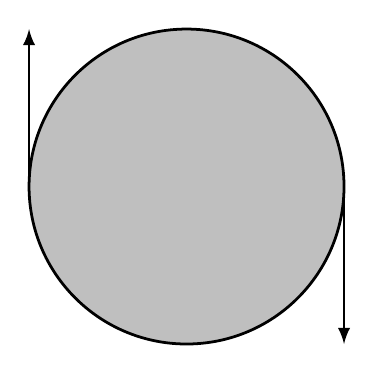
\begin{tikzpicture}
			\filldraw[color=black, fill=lightgray, line width=1pt] (0,0) circle (2);
			\draw[-latex, line width=1pt] (2,0) -- ++(0,-2);
			\draw[-latex, line width=1pt] (-2,0) -- ++(0,+2);
		\end{tikzpicture}
	}
	\caption{An opposite pair of forces applied on a round body.}
	\label{force-pair}
\end{figure}

In general, the net physical effect on a body can be broken down into a force and a torque.
Both of them are equivalently applied on the center of the mass, so that their exact position don't need to be explicitly taken care of.
Given a positioned force $(\mathbf{f}, \mathbf{r})$, where $\mathbf{f}$ is the force and $\mathbf{r}$ is the vector from the center of mass to the point of effect, the equivalent force-torque tuple on the center of mass can be calculated by the following formulae (\ref{positioned-force-to-force-torque-tuple}).

\begin{equation}
	(\mathbf{f},\mathbf{r})_{\text{positioned force}}
	\mapsto
	(\mathbf{f},\mathbf{r}\times\mathbf{f})_{\text{force-torque tuple}}.
	\label{positioned-force-to-force-torque-tuple}
\end{equation}

And to compose two force-torque tuples, simply sum them up component-wise (\ref{composing-two-force-torque-tuples}).

\begin{equation}
	(\mathbf{f}_1,\mathbf{\tau}_1)
	\oplus
	(\mathbf{f}_2,\mathbf{\tau}_2)
	=
	(\mathbf{f}_1+\mathbf{f}_2,\mathbf{\tau}_1+\mathbf{\tau}_2).
	\label{composing-two-force-torque-tuples}
\end{equation}

By applying this into formula (\ref{net-pressure-force}), the net water pressure force could then be calculated.